\chapter{Mengakses Basis Data NoSQL: mongoDB}

\section{Apa itu Basis Data NoSQL?}

\index{NOSQL}Pada awalnya, istilah NoSQL digunakan oleh Carlo Strozzi untuk menyebut nama software basis data yang dibuat olehnya. Software basis data tersebut tidak mengikuti standar SQL, sehingga dia menyebut software tersebut dengan "NoSQL"\footnote{\url{http://www.strozzi.it/cgi-bin/CSA/tw7/I/en_US/nosql/Home\%20Page}}. Setelah itu, istilah NoSQL dipopulerkan oleh Eric Evans untuk menyebut jenis software basis data yang tidak menggunakan standar SQL. Dalam perkembangan berikutnya, NoSQL ini lebih diarahkan pada "Not Only SQL" dan digunakan untuk kategorisasi basis data \textit{non-relational} (misalnya OODBMS, Graph Database, Document-oriented, dan lain-lain). Meski ada usaha untuk menstandarkan bahasa \textit{query} untuk NoSQL (UnQL - \textit{Unstructured Query Language}), sampai saat ini usaha tersebut tidak menghasilkan sesuatu hal yang disepakati bersama karena dunia NoSQL memang kompleks sekali. Untuk melihat daftar dari basis data NoSQL, anda bisa melihat ke \url{http://nosql-databases.org}.

\section{Mengenal mongoDB dan Fitur-fiturnya}

\index{mongoDB}mongoDB adalah salah satu software NoSQL yang termasuk dalam kategori \textit{Document Store} / \textit{Document-Oriented Database}, yaitu data disimpan dalam bentuk dokumen. Suatu dokumen bisa diibaratkan seperti suatu \textit{record} dalam basis data relasional dan isi dari masing-masing dokumen tersebut bisa berbeda-beda dan ada pula yang sama. Hal ini berbeda dengan basis data relasional yang menetapkan keseragaman kolom serta tipe data dengan data yang NULL jika tidak terdapat data. mongoDB menyimpan data dalam bentuk dokumen dengan menggunakan format JSON. Berikut adalah fitur dari mongoDB:
\begin{itemize}
	\item menggunakan format JSON dalam penyimpanan data
	\item mendukung indeks
	\item mendukung replikasi
	\item auto-sharding untuk skalabilitas horizontal
	\item query yang lengkap
	\item pembaruan data yang cepat
	\item mendukung Map/Reduce
	\item mendukung GridFS
\end{itemize}

\subsection{Memulai Server}
Seperti halnya basis data relasional seperti MySQL, PostgreSQL, dan lain-lain, mongoDB juga memulai dengan menjalankan server yang memungkinkan server tersebut melayani permintaan akses data dokumen melalui klien. Untuk memulai server, siapkan direktori yang akan menjadi tempat menyimpan data (defaultnya adalah /data/db). Jika menginginkan lokasi lain, gunakan argumen \textit{--dbpath} saat menjalankan server sebagai berikut (buat direktorinya jika belum ada):

\lstset{language=bash,caption=Menjalankan server MongoDB (mongod)}
\lstinputlisting{src/non-nodejs/bab-06/mongodb-run.txt}

Untuk mengakhiri server, tekan \textit{Ctrl-C}, mongoDB akan mengakhiri server sebagai berikut:

\lstset{language=bash,caption=Mengakhiri server MongoDB (mongod)}
\lstinputlisting{src/non-nodejs/bab-06/mongodb-stop.txt}

\subsection{Klien dan Shell mongoDB}

Setelah server hidup, pemrogram bisa menggunakan antarmuka administrasi web maupun menggunakan shell. \textit{Admin web console} bisa diakses menggunakan port 28017 seperti pada gambar~\ref{fig:mongowebadminconsole}. Sementara itu, untuk mengakses server menggunakan shell, bisa digunakan perintah \textit{mongo} sebagai berikut:

\lstset{language=bash,caption=Shell mongoDB (mongo)}
\lstinputlisting{src/non-nodejs/bab-06/mongodb-shell.txt}

  \begin{figure}
    \begin{center}
      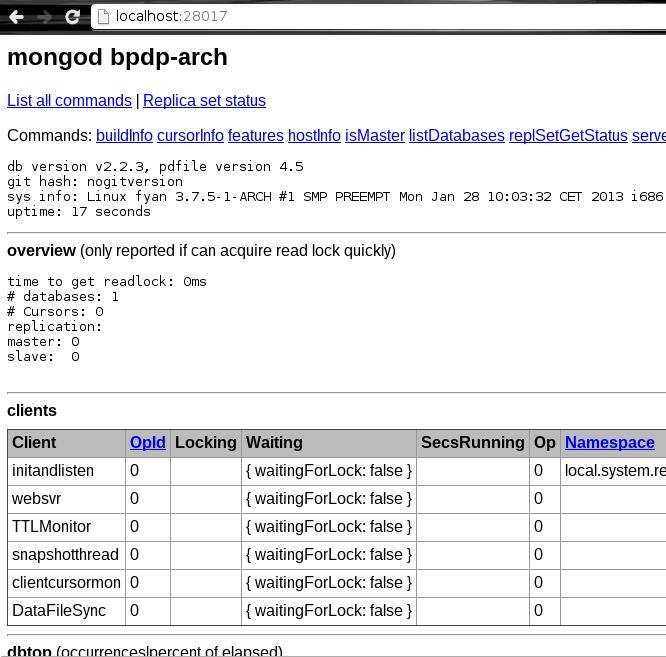
\includegraphics[scale=0.5]{images/mongodb-web-interface.jpg}
    \end{center}
    \caption{Admin web console untuk mongoDB}
    \label{fig:mongowebadminconsole}
  \end{figure}


\subsection{Documents dan Collections}

Konsep dasar yang harus dipahami dalam mongoDB sebagai \textit{document-oriented database} adalah \textit{documents} dan \textit{collections}. Sama halnya dengan basis data relasional, mongoDB menyimpan data dalam suatu basis data. Di dalam basis data tersebut terdapat \textit{collections} yang bisa diibaratkan seperti tabel dalam basis data relasional. \textit{Collections} digunakan untuk menyimpan dokumen (\textit{documents}). Dalam istilah basis data relasional, \textit{documents} adalah \textit{records}. Kerjakan latihan berikut untuk memahami pengertian dari \textit{documents} dan \textit{collections}.

\lstset{language=bash,caption=Sesi dalam shell mongoDB}
\lstinputlisting{src/non-nodejs/bab-06/mongodb-shell-session.txt}

Basis data mongoDB hanya akan dibuat jika sudah dilakukan perintah untuk menyisipkan atau mengisikan data \textit{documents} ke dalam \textit{collections} seperti perintah di atas.

\section{Node.js dan MongoDB}

\subsection{Node-gyp}

\index{Node-gyp}Node-gyp merupakan \textit{native add-on build tool}, berfungsi untuk membantu proses kompilasi modul add-on native di Node.js. Node-gyp merupakan software bebas dan bisa diinstall menggunakan npm:

\lstset{language=bash,caption=Instalasi node-gyp}
\lstinputlisting{src/non-nodejs/bab-06/install-node-gyp.txt}

Node-gyp ini diinstall pada lokasi global. Pada materi ini, Node-gyp diperlukan untuk membangun \textit{driver} dari mongoDB sehingga mongoDB bisa diakses oleh Node.js. 

\subsection{Driver Node.js untuk mongoDB}

\index{mongoDB!Driver}Mengakses mongoDB dari Node.js bisa dilakukan dengan menggunakan driver atau berbagai \textit{wrapper} serta solusi sejenis ORM \textit{Object-Relational Mapping}. Salah satu solusi yang tersedia adalah paket \textbf{mongodb}.

\lstset{language=bash,caption=Instalasi driver mongoDB}
\lstinputlisting{src/non-nodejs/bab-06/install-paket-mongodb.txt}

Solusi lain yang bisa digunakan antara lain adalah:
\begin{itemize}
	\item Mongoose (\url{http://mongoosejs.com/})
	\item Mongojs (\url{https://github.com/gett/mongojs})
	\item Mongolia (\url{https://github.com/masylum/mongolia})
	\item Mongoskin (\url{https://github.com/kissjs/node-mongoskin})
\end{itemize}

\subsection{Mengakses mongoDB dari Node.js}

Dengan menggunakan \textit{collections} dan \textit{documents} di atas, kita akan mengakses data tersebut menggunakan Node.js. Untuk lebih menyederhanakan, kita akan menggunakan \textit{wrapper} dari mongoDB native driver, yaitu Mongojs. Install Mongojs lebih dahulu menggunakan npm:

\lstset{language=bash,caption=Instalasi wrapper mongojs}
\lstinputlisting{src/non-nodejs/bab-06/install-paket-mongojs.txt}

Setelah itu, buat program sesuai dengan listing program berikut.

\lstset{language=bash,caption=Mengakses mongoDB dari Node.js}
\lstinputlisting{src/bab-06/akses-mongodb.js}

\section{Aplikasi Web Menggunakan Node.js dan mongoDB}

Contoh aplikasi web berikut hanya digunakan untuk mengambil data dari mongoDB kemudian menampilkannya di web. Data diambil dari basis data mongoDB yang sudah dibuat sebelumnya (mydb). Untuk keperluan ini, kita akan menggunakan framework Express (\url{http://expressjs.com}). Install Express di level global dengan \textit{npm install -g express}. Setelah terinstall, buat subdirektori baru (lokasi bebas) yang akan digunakan untuk menyimpan aplikasi web. Setelah itu, masuk ke direktori tersebut kemudian buat kerangka aplikasi di subdirektori tersebut menggunakan perintah ``express'' (lihat bab 1).

Berikut ini adalah beberapa perubahan yang dilakukan untuk rerangka aplikasi yang dihasilkan dari perintah \textit{express} tersebut.

\lstset{language=JavaScript,caption=Express+MongoDB web: app.js}
\lstinputlisting{src/bab-06/web/app.js}

\lstset{language=JavaScript,caption=Express+MongoDB web: package.json}
\lstinputlisting{src/bab-06/web/package.json}

\lstset{language=JavaScript,caption=Express+MonggoDB web: routes/index.js}
\lstinputlisting{src/bab-06/web/routes/index.js}

Selain itu, ada beberapa tambahan file (routes/employee.js dan views/employee.jade), penghapusan file (routes/user.js), dan perubahan yang cukup signifikan pada file \textit{views/index.jade}.

\lstset{language=JavaScript,caption=Express+MongoDB web: routes/employee.js}
\lstinputlisting{src/bab-06/web/routes/employee.js}

\lstset{language=html,caption=Express+MongoDB web: views/employee.jade}
\lstinputlisting{src/bab-06/web/views/employee.jade}

\lstset{language=html,caption=views/index.jade}
\lstinputlisting{src/bab-06/web/views/index.jade}
